\documentclass[10pt,a4paper]{article}

% Coursebook format: 10pt Times New Roman, double spaced, A4, 1 inch margins, numbered pages
\usepackage[a4paper,margin=1in]{geometry}
\usepackage[T1]{fontenc}
\usepackage{newtxtext,newtxmath}
\usepackage{setspace}
\usepackage{graphicx}
\usepackage{tabularx}
\usepackage{booktabs}
\usepackage{array}
\usepackage{enumitem}
\usepackage{listings}
\usepackage{xcolor}
\usepackage{caption}
\usepackage{url}
\usepackage[hidelinks]{hyperref}

\usepackage[compact]{titlesec}
\titlespacing*{\section}{0pt}{8pt}{2pt}
\titlespacing*{\subsection}{0pt}{6pt}{0pt}

% let LaTeX put more floats on a page instead of leaving gaps
\renewcommand{\topfraction}{0.9}
\renewcommand{\bottomfraction}{0.8}
\renewcommand{\textfraction}{0.1}
\renewcommand{\floatpagefraction}{0.8}
\setlength{\textfloatsep}{8pt}
\setlength{\intextsep}{8pt}

\captionsetup{font=small,labelfont=bf,skip=4pt}
\setlist{nosep}
\renewcommand{\arraystretch}{1.2}
\newcolumntype{L}{>{\raggedright\arraybackslash}X}

\lstset{
  basicstyle=\ttfamily\footnotesize,
  backgroundcolor=\color{gray!8},
  frame=single,
  rulecolor=\color{gray!40},
  columns=fullflexible,
  keepspaces=true,
  showstringspaces=false,
  aboveskip=6pt,
  belowskip=6pt
}

\begin{document}

% ---------------------------------------------------------------- cover page + table of contents
\thispagestyle{empty}
\begin{center}
  \vspace*{0.5cm}
  {\LARGE\bfseries Decentralized Identity and Consent Management\\[4pt] for Healthcare ID Verification\par}
  \vspace{0.6cm}
  {\large BCS3210 Blockchains, Maastricht University, 2026--2027\par}
  \vspace{0.2cm}
  {\large Group 21 \quad October 2026\par}
  \vspace{0.6cm}
  \begin{tabular}{ll}
    \toprule
    \textbf{Student name} & \textbf{Student ID} \\
    \midrule
    Sam Prior     & i6384844 \\
    Gyorgy Balint & i6379606 \\
    Luka Toplak   & i6380097 \\
    Jack Bikar    & i6347337 \\
    \bottomrule
  \end{tabular}
\end{center}
\vspace{0.6cm}
\begin{singlespace}
\tableofcontents
\end{singlespace}
\clearpage

\setcounter{page}{1}
\doublespacing

% ================================================================ 1
\section{Introduction}

\subsection{Problem Statement}

Before providing care, healthcare organisations often need to verify a patient's identity, usually by checking a government-issued document such as a passport or national identity card. In practice, a copy or scan of that document may then be stored in the databases of hospitals, clinics, laboratories, insurers or other healthcare providers.

This creates a few problems. First, the same sensitive identity document can be copied and stored in many different systems, and every database that stores it becomes another possible target for a data breach, unauthorised access or accidental disclosure~\cite{hipaa}. Second, patients often have limited control over their information after giving it to a provider. They may not know exactly who accessed their document, when it was accessed or how long it remains available, and it may be difficult to withdraw that permission once a copy has already been stored. Third, healthcare providers may keep internal logs, but these are controlled by the organisation itself and are not always visible to the patient, so it may be difficult to prove who accessed a document and whether they had permission at the time.

These issues are especially important in healthcare because both identity documents and health information are highly sensitive. Healthcare organisations must protect this information and follow data-protection requirements such as the General Data Protection Regulation (GDPR)~\cite{gdpr}. At the same time, they still need a practical way to verify that a patient is who they claim to be.

\subsection{Existing Systems and Research Gap}

A common approach is the traditional healthcare database, where hospitals, clinics and other providers keep their own copies of patient documents, so the same sensitive information can end up stored in several places. Self-sovereign identity systems try to give more control back to the user with a digital wallet that shares only the information needed~\cite{eidas,eudi,w3cvc}, but they are often general-purpose and do not always deal with giving a hospital temporary access to an off-chain identity document that the patient can revoke later. Blockchain-based healthcare data-sharing systems use blockchain to keep a record of who shared or requested data, and smart contracts to manage permissions~\cite{medrec,ancile}. However, healthcare data is sensitive, so putting full identity documents or medical records directly on a public blockchain would not be a good idea. The main gap is that these features are not always combined in one place. Our project combines these ideas in one prototype, giving the patient more control while still allowing healthcare organisations to verify the document and request access in a clear and traceable way.

\subsection{Our Approach and Objectives}

This project proposes a decentralised identity and data-sharing platform for government-ID verification in healthcare. The system uses smart contracts on an Ethereum-compatible blockchain to manage identity registration, consent, access logging and token rewards. The objectives of this project are to:
\begin{itemize}
  \item allow patients to register a digital identity while keeping their government-ID documents off-chain, with only a document link and cryptographic hash stored on-chain;
  \item allow patients to grant consent to a specific requester for a limited time and to revoke it before it expires;
  \item allow requesters to access a document only when valid consent exists;
  \item record all access attempts, including both granted and denied attempts, in an immutable audit log;
  \item reward patients with tokens for granting consent without making personal data something that can be bought or sold;
  \item test the smart contracts, measure the gas cost of the main functions and simulate multiple patients, requesters and administrators using the system.
\end{itemize}

The system is designed as a proof of concept rather than a complete production healthcare platform. It does not remove the need for secure off-chain storage, identity verification procedures, legal agreements or compliance with healthcare and data-protection rules.

% ================================================================ 2
\section{Architecture}

\subsection{System Overview}

Our platform is made up of four smart contracts, deployed on a local Ethereum network, and one off-chain component that we call the patient's vault (Figure~\ref{fig:architecture}). Instead of putting all the logic into one large contract, we gave each contract a single responsibility and let them communicate through small interfaces. This made each contract easier to test on its own and easier to change without breaking the others.

\begin{figure}[htbp]
  \centering
  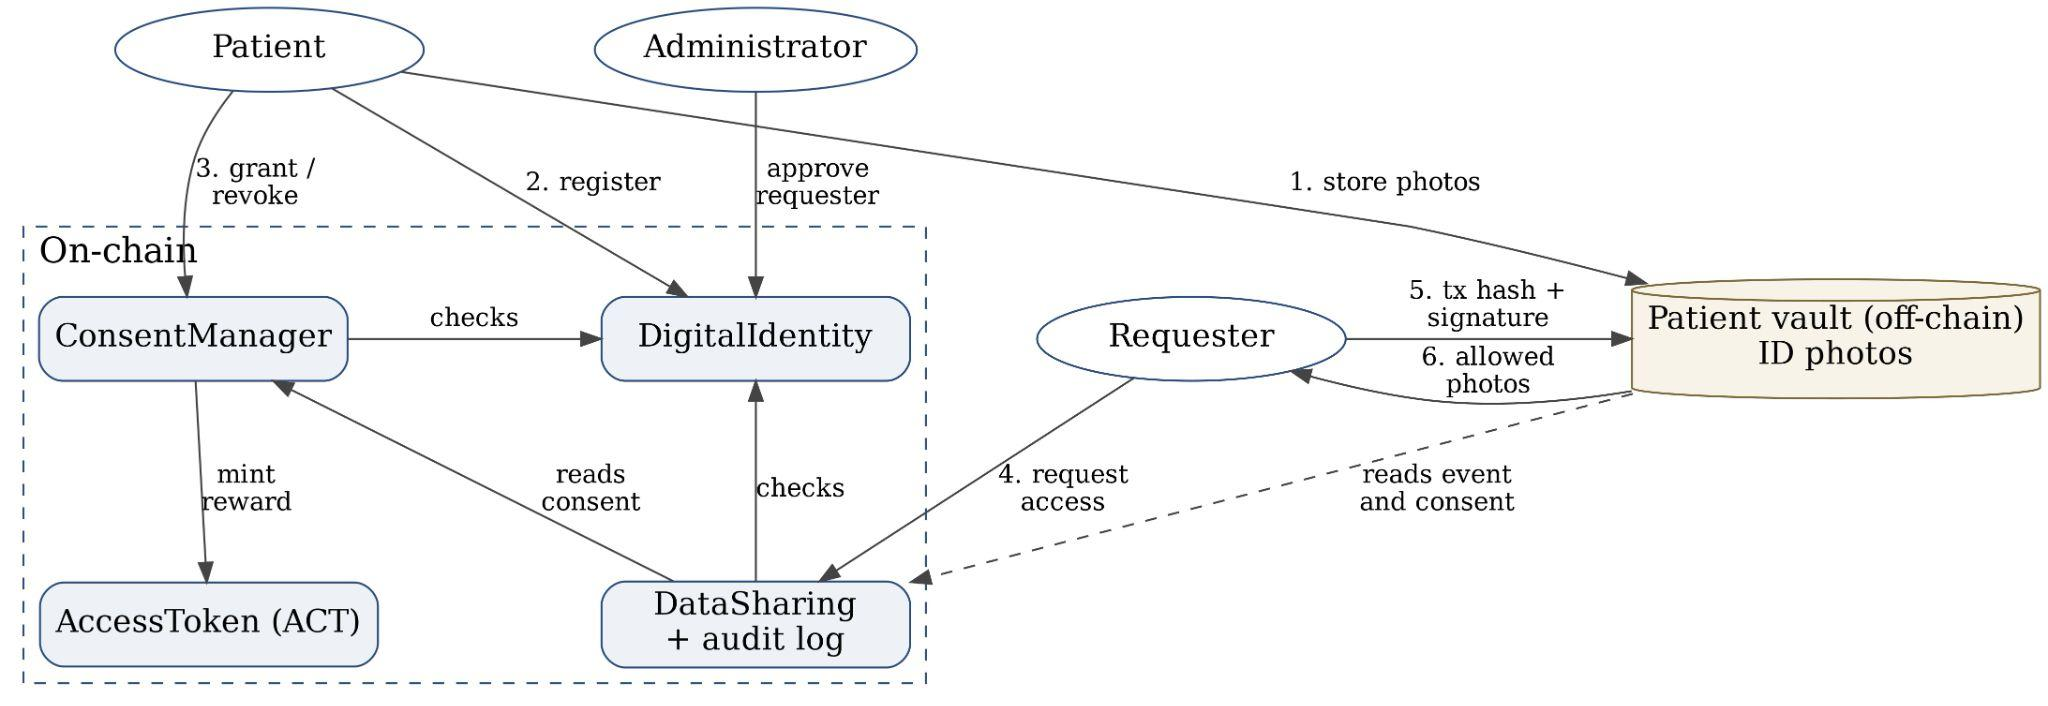
\includegraphics[width=0.85\linewidth]{figures/architecture.jpg}
  \caption{Components of the platform and their interaction.}
  \label{fig:architecture}
\end{figure}

The \texttt{DigitalIdentity} contract handles patient registration and keeps track of which requesters have been approved by the administrator. The \texttt{ConsentManager} stores the consents that patients give to requesters and checks whether a given consent is still valid. \texttt{DataSharing} is the contract that requesters actually interact with: it receives access requests, decides whether they should be granted and records every attempt in an audit log. Finally, \texttt{AccessToken} is an ERC-20 token (ACT) used to reward patients for giving consent, and only the \texttt{ConsentManager} is allowed to mint new tokens.

The vault is a small program on the patient's side that stores the actual ID photos. We needed it because a smart contract cannot keep data secret, since anything stored on a public blockchain can be read by anyone. So the work is split: the contracts decide who is allowed to access the documents, and the vault decides whether to release the files, using proof from the blockchain that access was granted.

\subsection{User Roles and Permissions}

The system has three roles. Each one can only perform the actions it needs (Table~\ref{tab:roles}).

\begin{table}[htbp]
  \centering
  \footnotesize
  \begin{tabularx}{\linewidth}{>{\raggedright\arraybackslash}p{3.2cm}LL}
    \toprule
    \textbf{Role} & \textbf{Can} & \textbf{Cannot} \\
    \midrule
    Patient (identity owner) & Register, update document hashes, grant and revoke consent, read own audit log & Grant consent on behalf of someone else, change or delete the log \\
    Requester (doctor, hospital, lab, insurer) & Request access, receive allowed photos from the vault, check their hashes & Access without valid consent, give itself consent \\
    Administrator (platform operator) & Approve or remove requesters, change the reward amount, pause data sharing & See the documents, grant or revoke consent, delete log entries \\
    \bottomrule
  \end{tabularx}
  \caption{Roles and permissions.}
  \label{tab:roles}
\end{table}

We deliberately kept the administrator out of the data path, so it never sees the documents and cannot grant or revoke consent on anyone's behalf. Its only job is to approve which addresses belong to real healthcare providers, so a patient cannot accidentally share their ID with an unknown address.

\subsection{Data Model: On-chain vs Off-chain}

Anything stored on a public blockchain can be read by anyone and can never be deleted. If we put personal data on-chain, it would be exposed permanently, which would also conflict with the GDPR right to erasure~\cite{gdpr}. We therefore followed a simple rule: anything that can identify a person stays off-chain, and only hashes, references and permission records are stored on-chain (Table~\ref{tab:data}).

\begin{table}[htbp]
  \centering
  \footnotesize
  \begin{tabularx}{\linewidth}{Lllp{4.2cm}}
    \toprule
    \textbf{Attribute} & \textbf{On-chain} & \textbf{Off-chain} & \textbf{Hashed} \\
    \midrule
    Wallet address of patient / requester & Yes & No & No (already a pseudonym) \\
    Name, date of birth, ID number & No & Yes (vault) & No \\
    Email & Hash only & Yes & Yes, with a salt kept by the patient \\
    Front and back photo of the ID & Hash only & Yes (vault) & Yes, SHA-256 \\
    Storage reference to the vault & Yes & Points to vault & No \\
    Consent (scope, start, end, revoked) & Yes & No & No \\
    Access log entry (requester, time, result, reason) & Yes & No & No \\
    ACT token balance & Yes & No & No \\
    \bottomrule
  \end{tabularx}
  \caption{Where each attribute is stored.}
  \label{tab:data}
\end{table}

Storing the photo hashes lets a requester check that the photos they receive are exactly the ones the patient registered, since any change to a photo would produce a different hash. We added a salt to the email hash because email addresses are easy to guess: without a salt, an attacker could hash a list of common emails and compare the results with the on-chain value.

\subsection{Consent and Incentives}

Each consent is given by a patient to one specific approved requester. It has a scope, which defines which part of the document can be shared (front only, back only or both), and a duration between 1 and 365 days. Only the patient can grant or revoke their own consents, and granting again to the same requester replaces the old consent.

At any point, a consent is in one of four states: no consent, active, revoked or expired (Figure~\ref{fig:states}). Revoking takes effect immediately. For expiry, we chose a lazy approach: nothing happens on-chain when a consent runs out. Instead, every check compares the current time with the stored end time, so nobody has to pay gas just to clean up expired consents.

\begin{figure}[htbp]
  \centering
  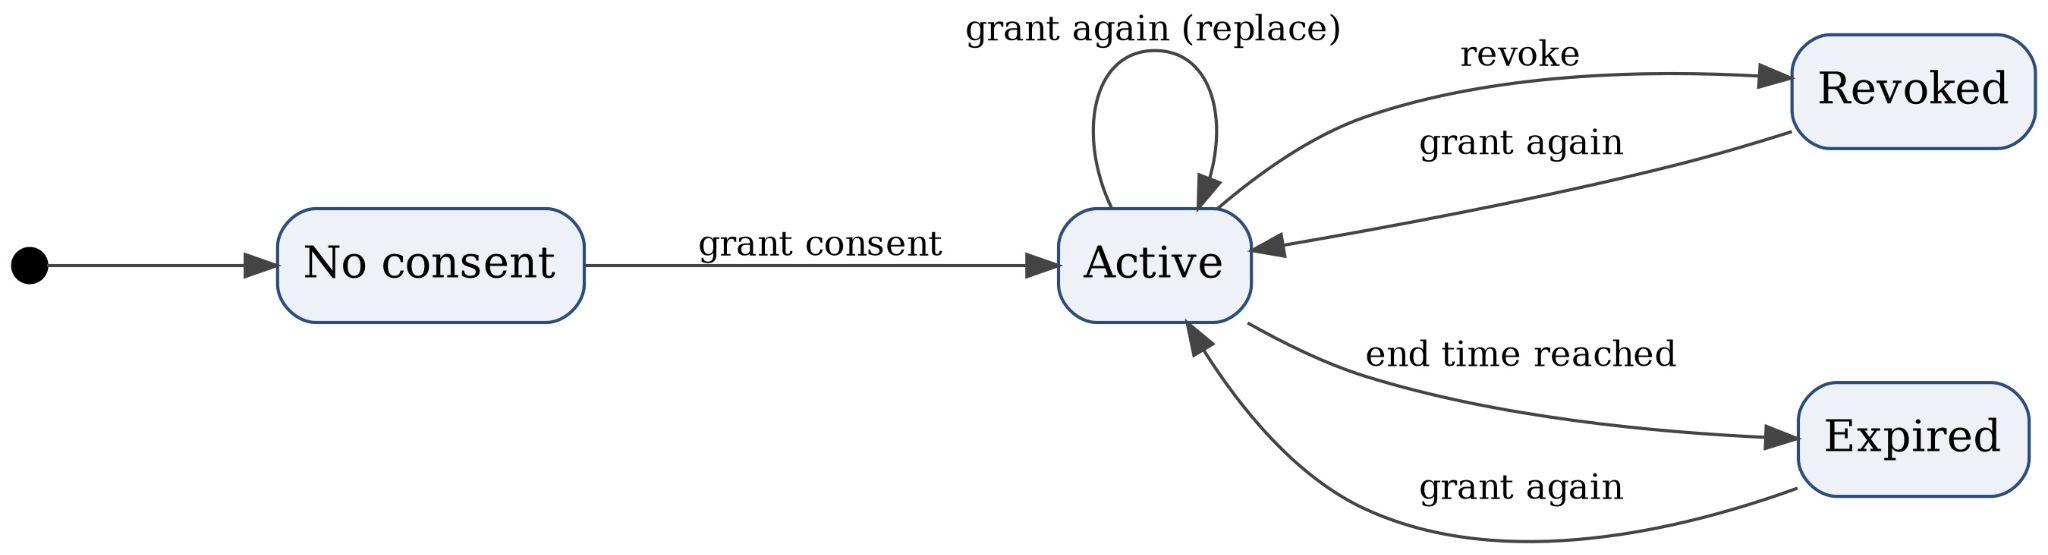
\includegraphics[width=0.55\linewidth]{figures/consent-states.jpg}
  \caption{Lifecycle of a consent.}
  \label{fig:states}
\end{figure}

Patients receive 10 ACT the first time they give consent to a requester. Later consents to the same requester are not rewarded, because otherwise a patient could keep granting and revoking consent just to collect tokens. The token is only meant as a reward for taking part. It is never checked when access is requested and never moves during data access, so it cannot be used to buy access to someone's data.

\subsection{Access Flow and Audit Log}
\label{sec:accessflow}

Figure~\ref{fig:access} shows how a requester obtains the photos. First, the requester sends an access request to the \texttt{DataSharing} contract. The contract checks whether the requester is approved and whether a valid consent exists. It then records the attempt in the patient's audit log and emits either a ``granted'' or a ``denied'' event, together with a reason (not approved, no consent, revoked or expired).

\begin{figure}[htbp]
  \centering
  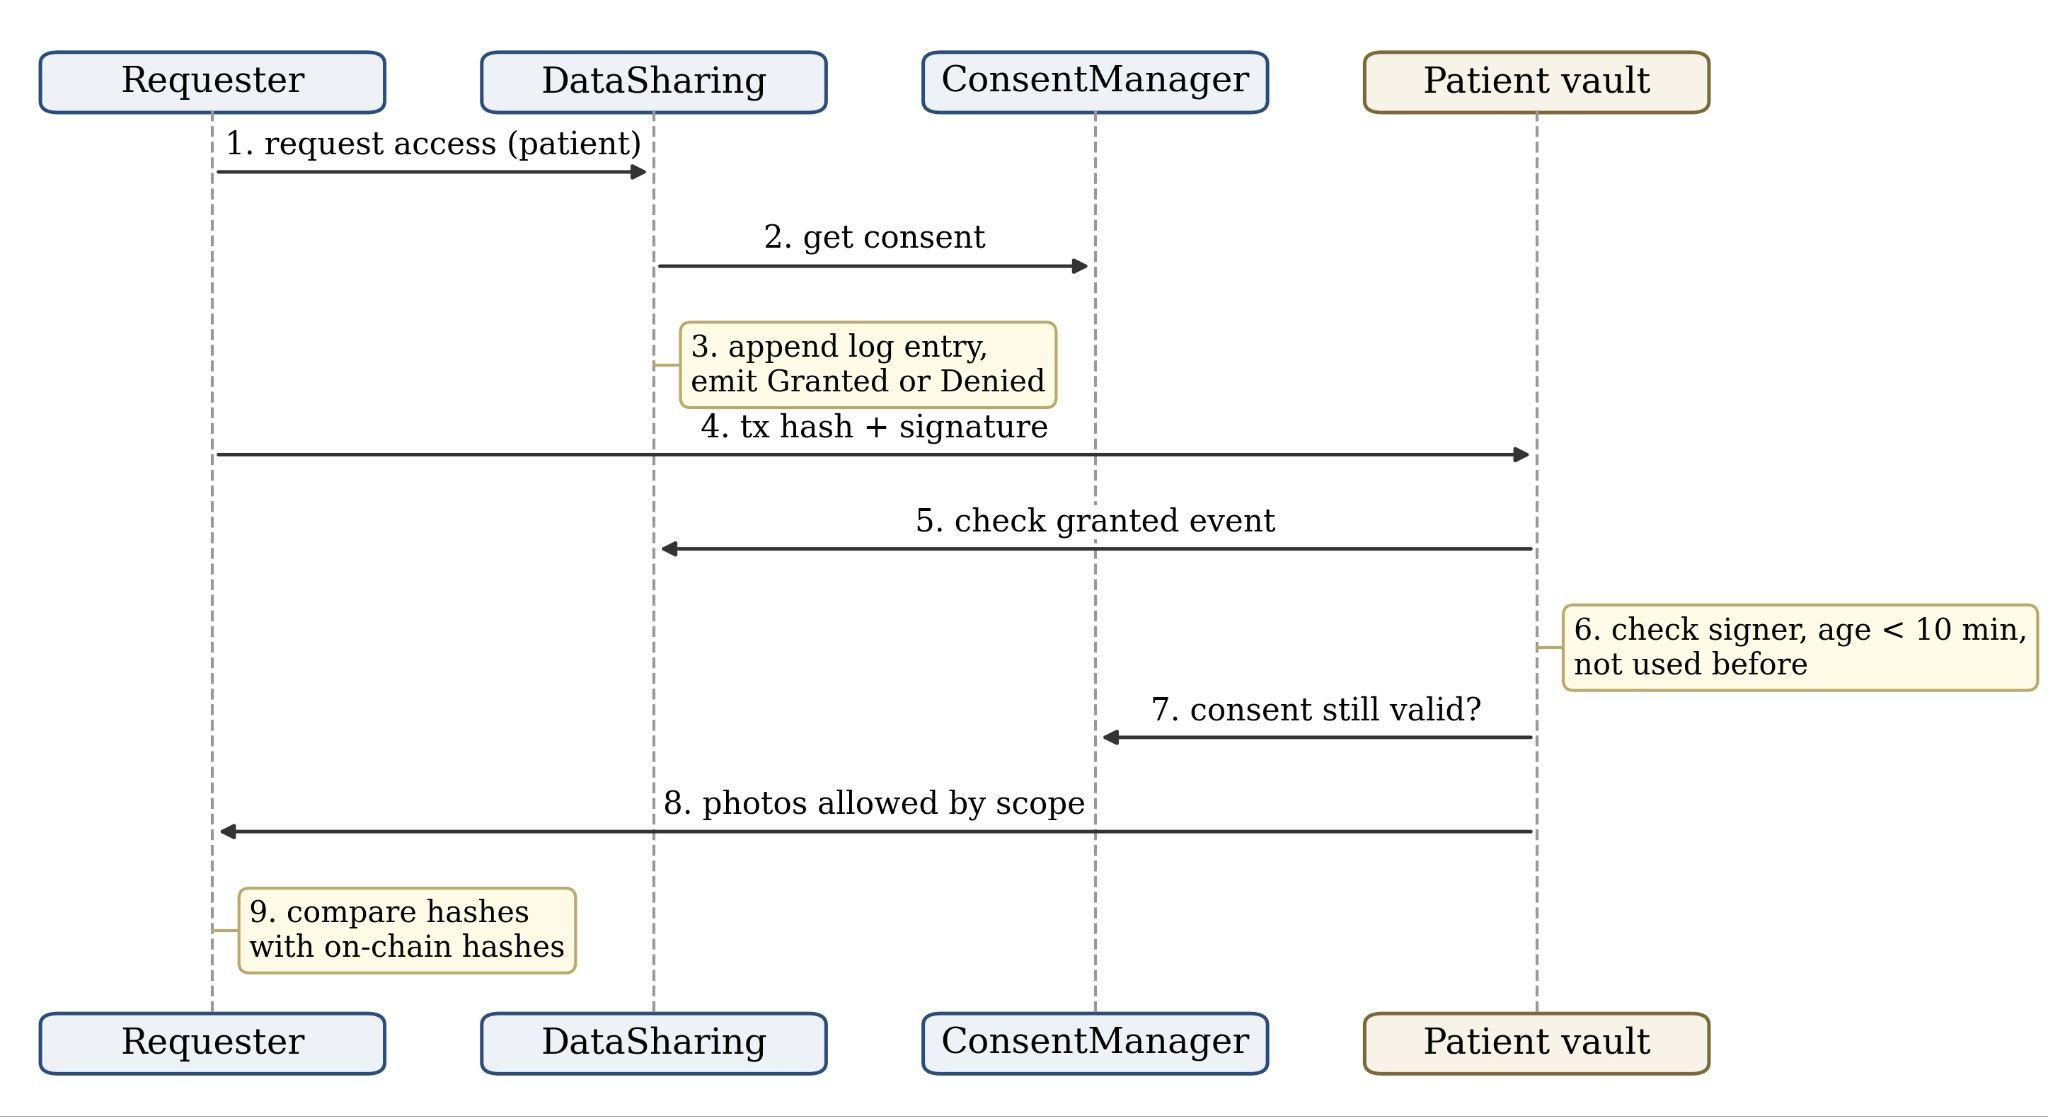
\includegraphics[width=0.5\linewidth]{figures/access-flow.jpg}
  \caption{Access request and file release by the vault.}
  \label{fig:access}
\end{figure}

One of our most important design decisions was that a denied request does not revert. In Ethereum, a revert undoes every change made in the transaction, including the log entry, so failed attempts would leave no trace at all. Instead, the contract always writes the log entry and simply reports the request as denied. The only exception is a request for an address that is not a registered patient, which is rejected straight away. Since there is no function to edit or delete log entries, the log is append-only. The log can be read by anyone, but we considered this acceptable because it only contains addresses and timestamps, not personal data.

After a granted request, the requester sends the transaction hash and a signature over it to the patient's vault. The vault checks this request against the blockchain (Section~\ref{sec:offchain}) and only then releases the photos allowed by the scope. The requester then hashes the received photos and compares them with the hashes stored on-chain. Since the vault only responds to granted on-chain requests, every download has a matching entry in the audit log.

\subsection{Assumptions}

Our design assumes that the administrator only approves real healthcare providers, that the patient's vault is online and stores the photos securely, and that requesters keep their private keys safe, since their signature proves their identity to the vault. The system runs on a local Hardhat network, where transactions are confirmed immediately and gas has no real cost. We discuss what these assumptions mean for a real deployment in Section~\ref{sec:discussion}.

% ================================================================ 3
\section{Implementation}
\label{sec:implementation}

For the Ethereum simulation we used Hardhat 3, Solidity 0.8.28 (optimizer on, 200 runs) for the contract code, forge-std for tests and Hardhat Ignition for deployment. The off-chain code, which runs on the clients' devices, is written in Python with web3.py.

\subsection{Smart Contracts}

We wrote the owner logic and the ERC-20 token ourselves instead of importing OpenZeppelin. OpenZeppelin would have meant less code, but we wanted to stay close to how things were done in the course. Access control is the usual \texttt{onlyOwner}-style modifiers plus role mappings, and every input is checked with a \texttt{require} and a short error message (e.g.\ ``Duration must be 1-365 days'').

The function that needed the most thought was \texttt{requestAccess}, because of the logging requirement from Section~\ref{sec:accessflow}. It only reverts if the patient is not registered at all. In every other case it works out a reason, writes the log entry, emits an event and returns true or false:

\begin{lstlisting}
if (!identity.isApprovedRequester(msg.sender)) reason = Reason.NotApproved;
else if (!exists) reason = Reason.NoConsent;
else if (revoked) reason = Reason.Revoked;
else if (block.timestamp >= expiresAt) reason = Reason.Expired;
granted = (reason == Reason.None);   // log + event in both cases, no revert
\end{lstlisting}

Deployment is a single Ignition module. It deploys the token, the identity contract, the consent manager and data sharing in that order, since the later contracts need the addresses of the earlier ones. The last step is \texttt{setMinter}, which makes the consent manager the only contract that can mint ACT.

\subsection{Off-chain Components}
\label{sec:offchain}

The Python code is in \texttt{offchain/} and has three parts. The hashing tool computes the SHA-256 of the ID photos and the salted email hash. The second part generates fake patients and ID images, so we never needed real personal data. The third part is the vault.

The vault is where access control for the files really happens. A requester sends it the hash of its \texttt{requestAccess} transaction plus a signature over that hash, and the vault checks that:
\begin{itemize}
  \item the transaction went to \texttt{DataSharing} and emitted \texttt{AccessGranted} for this patient,
  \item the signer recovered from the signature is the requester of that transaction,
  \item the request is at most 10 minutes old,
  \item the same transaction hash was not used before,
  \item the consent is still valid (the patient may have revoked it after the request).
\end{itemize}
Only if all five pass does it copy the photos that the scope allows. The time limit and the used-before check stop someone from replaying an old or copied request. On the other side, the requester hashes the files it got and compares them with the hashes on-chain, so a changed photo is noticed.

% ================================================================ 4
\section{Experimental Results}

\subsection{Test Setup}

The contracts were tested on a local Hardhat network with the setup described in Section~\ref{sec:implementation}. The unit and integration tests were written in Solidity. We used generated addresses and fake document hashes throughout the tests, so no real patient data was used.

We ran the tests with \texttt{npx hardhat test} and measured gas usage with \texttt{npx hardhat test --gas-stats} and \texttt{scripts/gas-report.ts}.
For the multi-user simulation, we ran \texttt{scripts/simulate.ts} against a local Hardhat node, measuring the time between sending each transaction and receiving its receipt.

\subsection{Unit Tests}

We ran 60 unit tests, and all 60 passed with no failures. Table~\ref{tab:tests} shows the test count per contract, what the tests were checking and why they matter.

\begin{table}[htbp]
  \centering
  \footnotesize
  \begin{tabularx}{\linewidth}{>{\raggedright\arraybackslash}p{2.4cm}LLr}
    \toprule
    \textbf{Contract} & \textbf{Main checks} & \textbf{Why it matters} & \textbf{Passed} \\
    \midrule
    \texttt{AccessToken} & Minting permissions, transfers, approvals, insufficient balance and allowance & If anyone could mint, the reward would be worthless and could be abused & 10/10 \\
    \texttt{DigitalIdentity} & Registration, input validation, document updates and requester approval permissions & Wrong or empty hashes would make the integrity check of the photos useless & 16/16 \\
    \texttt{ConsentManager} & Consent scope, duration, revocation, expiry and token rewards & Access must follow the patient's choices and end when it should; patients must not farm tokens by granting and revoking consent & 21/21 \\
    \texttt{DataSharing} & Access decisions, audit logs, events and pause permissions & Denied requests must be logged without reverting, as reverting would erase the audit entry & 13/13 \\
    \midrule
    \textbf{Total} & All unit tests & & \textbf{60/60} \\
    \bottomrule
  \end{tabularx}
  \caption{Unit test results.}
  \label{tab:tests}
\end{table}

We also tested the consent boundaries. Durations of 1 and 365 days were accepted, while 0 and 366 were rejected. Consent remained valid until one second before its expiry timestamp. A duration fuzz test passed across 256 random runs.

\subsection{Integration Test}

The full workflow was tested to check that the four contracts work together as intended. A patient registered their identity and granted consent to an approved requester, and the requester successfully requested access. The patient then revoked consent, and the next access request was denied. The same test also checked access before consent was granted and after a re-granted consent expired, and both requests were denied. The workflow test passed and produced five audit entries, recording both granted and denied attempts.

\subsection{Gas Costs}

The deployment and transaction gas was measured using \texttt{scripts/gas-report.ts} on the Hardhat network. The script used 10 patients and two requesters. Tables~\ref{tab:deploy} and~\ref{tab:gas} show the costs after optimisation.

\begin{table}[htbp]
  \centering
  \footnotesize
  \begin{minipage}[t]{0.40\linewidth}
    \centering
    \vspace{0pt}
    \begin{tabular}{lr}
      \toprule
      \textbf{Deployment / setup} & \textbf{Gas} \\
      \midrule
      \texttt{AccessToken} & 721,687 \\
      \texttt{DigitalIdentity} & 850,665 \\
      \texttt{ConsentManager} & 774,213 \\
      \texttt{DataSharing} & 774,276 \\
      Setting the token minter & 47,302 \\
      \midrule
      \textbf{Total} & \textbf{3,168,143} \\
      \bottomrule
    \end{tabular}
    \caption{Deployment and setup gas costs.}
    \label{tab:deploy}
  \end{minipage}\hfill
  \begin{minipage}[t]{0.57\linewidth}
    \centering
    \vspace{0pt}
    \begin{tabular}{lr}
      \toprule
      \textbf{Function or operation} & \textbf{Avg.\ gas} \\
      \midrule
      Approve requester & 49,686 \\
      Register patient & 145,921 \\
      Grant consent with first reward & 94,835 \\
      Re-grant consent without reward & 39,283 \\
      Revoke consent & 28,969 \\
      Request access: granted & 70,108 \\
      Request access: denied, first audit entry & 87,290 \\
      Request access: denied, revoked consent & 70,210 \\
      Request access: denied, unapproved requester & 63,413 \\
      Update document & 39,364 \\
      \bottomrule
    \end{tabular}
    \caption{Average gas cost per operation after optimisation.}
    \label{tab:gas}
  \end{minipage}
\end{table}

Since writing a new storage slot is one of the most expensive operations in the EVM~\cite{yellowpaper,eip2929}, the optimisation focused on storage writes: timestamps are stored as \texttt{uint64}, so that a consent and a log entry each fit into a single 32-byte storage slot~\cite{soliditydocs}. Optimisation reduced the average cost of granted access from 107,429 to 70,108 gas, a 34.7\% reduction. The first consent grant fell from 187,290 to 94,835 gas, a 49.4\% reduction. Deployment and setup costs increased by 0.9\%, but this was a one-time cost, while the savings applied to repeated operations. All 64 tests still passed after these changes.

\subsection{Multi-user Simulation}
\label{sec:simulation}

The platform was simulated with 5, 10, 20, 50 and 100 patients. Each run used fresh contracts, one administrator and one requester for every five patients. Patients registered, granted consent and received an access request. Around half then revoked consent before a second request, allowing us to simulate both granted and denied access. Transactions were submitted sequentially. Table~\ref{tab:sim} shows the results.

\begin{table}[htbp]
  \centering
  \footnotesize
  \begin{tabular}{rrrrr}
    \toprule
    \textbf{Patients} & \textbf{Requesters} & \textbf{Transactions} & \textbf{Total gas} & \textbf{Total time (s)} \\
    \midrule
    5   & 1  & 24  & 2,143,847  & 0.27 \\
    10  & 2  & 47  & 4,224,675  & 0.47 \\
    20  & 4  & 94  & 8,415,198  & 0.85 \\
    50  & 10 & 235 & 20,987,175 & 1.97 \\
    100 & 20 & 470 & 41,939,790 & 3.80 \\
    \bottomrule
  \end{tabular}
  \caption{Multi-user simulation results.}
  \label{tab:sim}
\end{table}

As patient numbers increased, total gas usage and runtime increased roughly proportionally, while gas per operation stayed the same as in Table~\ref{tab:gas}. Most transactions took around 8--10\,ms on the local node. These timings do not reflect public-network confirmation times because transactions were mined immediately.

% ================================================================ 5
\section{Discussion and Conclusion}
\label{sec:discussion}

\subsection{Discussion}

When it comes to performance, our local node confirms a transaction in a few milliseconds, but on Ethereum mainnet a block takes about 12 seconds and every request costs a fee, so Section~\ref{sec:simulation} shows the best case. Deploying on a Layer-2 rollup would bring the cost down.

When it comes to privacy, anyone can read the chain, so anyone can see which requester asked about which patient address, and when. The addresses are pseudonymous, but a pattern of visits can still say a lot on its own, although nobody can see the ID documents themselves.

When it comes to the administrator user, they alone decide which requesters are approved; in a real deployment the administrator would be the government, and the institutions would not be legally allowed to save copies, as this is the core trust that the project relies on. The blockchain can prove that access happened, not that the copy was deleted afterwards. Smaller things we would still fix are encrypting the files for the requester during transfer and using a wallet like MetaMask instead of the Hardhat test keys. The ACT token also has no real value yet, so for now the reward is mostly symbolic.

\subsection{Conclusion}

Looking back at the requirements, the platform fits them well: the ID photos stay with the patient, consent is scoped, time-limited and revocable, every access attempt is logged, only requesters with valid consent get the files, and the ACT reward never gives access to anything. A small set of smart contracts was enough to give patients control over who sees their ID documents and a record of every attempt, at about 70,000 gas per access request after optimisation. In our simulation, cost and time grew linearly with the number of users. The big lessons we learned were that a contract cannot log a failed attempt if the transaction reverts, and that it cannot keep anything secret, so the real access control for the files has to happen off-chain, based on proofs from the chain.

% ================================================================ 6
\section{Contribution Statement and Use of Generative AI}

\subsection*{Contribution Statement}

\begin{itemize}
  \item Sam Prior: [to be filled in]
  \item Gyorgy Balint: [to be filled in]
  \item Luka Toplak: [to be filled in]
  \item Jack Bikar: [to be filled in]
\end{itemize}

\subsection*{AI Use Statement}

We used generative AI (Claude, Anthropic) for: summarising the course material, reviewing a first version of our design, drafting the contract code, tests, scripts and the Python vault, and drafting parts of the text of the step deliverables and this report. The parts of our work affected are the code in the repository and the written deliverables. We have reviewed, run and tested all code, checked the numbers against our own measurements and the references against their sources, and we take responsibility for the submitted work. [Adjust this statement to your actual use before submission.]

% ================================================================ references
\begin{singlespace}
\small
\begin{thebibliography}{10}

\bibitem{hipaa}
The HIPAA Journal, ``Change Healthcare Responding to Cyberattack'', \url{https://www.hipaajournal.com/change-healthcare-responding-to-cyberattack/} (accessed 30 Sep 2026).

\bibitem{gdpr}
Regulation (EU) 2016/679 (General Data Protection Regulation), Art.~9 and Art.~17.

\bibitem{eidas}
Regulation (EU) No 910/2014 on electronic identification and trust services (eIDAS).

\bibitem{eudi}
Regulation (EU) 2024/1183 establishing the European Digital Identity Framework.

\bibitem{w3cvc}
W3C, ``Verifiable Credentials Data Model v2.0'', W3C Recommendation, 2025.

\bibitem{medrec}
A.~Azaria, A.~Ekblaw, T.~Vieira, A.~Lippman, ``MedRec: Using Blockchain for Medical Data Access and Permission Management'', 2nd International Conference on Open and Big Data (OBD), 2016.

\bibitem{ancile}
G.~G.~Dagher, J.~Mohler, M.~Milojkovic, P.~B.~Marella, ``Ancile: Privacy-preserving framework for access control and interoperability of electronic health records using blockchain technology'', Sustainable Cities and Society, vol.~39, pp.~283--297, 2018.

\bibitem{yellowpaper}
G.~Wood, ``Ethereum: A Secure Decentralised Generalised Transaction Ledger'' (Yellow Paper).

\bibitem{eip2929}
V.~Buterin, M.~Swende, ``EIP-2929: Gas cost increases for state access opcodes'', 2020.

\bibitem{soliditydocs}
Solidity documentation, ``Layout of State Variables in Storage'', \url{https://docs.soliditylang.org}.

\end{thebibliography}
\end{singlespace}

\end{document}
